\documentclass[conference]{IEEEtran}
\usepackage{graphicx}
\usepackage{booktabs}
\usepackage{amsmath}
\usepackage{url}
\usepackage{cite}
\graphicspath{{figures/}}

\title{Weather Conditions and LoRa Link Metrics: A Retrospective Analysis of Co-Located Measurements}

\author{\IEEEauthorblockN{TODO: Author Name(s)}
\IEEEauthorblockA{TODO: Affiliation, City, Country\\
TODO: Email address(es)}}

\begin{document}
\maketitle

\begin{abstract}
This paper reconstructs an exploratory study of associations between local weather observations and Long Range (LoRa) link measurements. The repository contains 1,059 LoRa records and 14,494 weather records spanning December 17, 2024 to January 2, 2025. A timestamp-window procedure matched 1,058 LoRa records to weather observations within $\pm5$~s. The resulting data contain received signal strength indicator (RSSI), signal-to-noise ratio (SNR), throughput, latency, and scalar meteorological variables. The strongest reproduced individual Pearson correlations were between cumulative/absolute rain readings and RSSI ($r=0.386$), SNR ($r=0.450$), and throughput ($r=0.312$). All individual correlations with latency were weak ($|r|\leq0.084$). On a fixed random holdout, the best recorded RSSI model among the tested configurations was degree-two polynomial regression ($R^2=0.190$), while the best SNR and throughput configurations were Lasso regression ($R^2=0.208$ and $0.118$, respectively). Every latency model had negative holdout $R^2$. These results indicate limited predictive performance and do not establish causality. Ambiguities in sensor units, sampling protocol, duplicated weather records, temporal dependence, and vector-valued weather fields constrain interpretation.
\end{abstract}

\begin{IEEEkeywords}
LoRa, weather, RSSI, SNR, throughput, latency, regression, wireless sensing
\end{IEEEkeywords}

\section{Introduction}
Long Range (LoRa) links are used in low-power sensing systems, but propagation and application-level performance may vary with environmental conditions. The analyzed repository investigates whether co-located weather measurements are associated with four observed LoRa metrics: received signal strength indicator (RSSI), signal-to-noise ratio (SNR), throughput, and latency.

The reconstructed research objective is to quantify those associations and evaluate whether standard regression models can predict each link metric from weather variables. The code implies the working hypothesis that weather measurements contain predictive information about LoRa performance. No preregistered hypothesis, protocol, or significance criterion is present; accordingly, this paper treats the work as retrospective and exploratory.

The contribution is an evidence-constrained reconstruction of the existing pipeline: (i) timestamp-window fusion of packet and weather logs; (ii) Pearson correlation screening; and (iii) holdout evaluation of linear, regularized, polynomial, nearest-neighbor, and random-forest regressors. The results show modest associations for RSSI, SNR, and throughput, but weak out-of-sample prediction and no useful latency prediction. They should not be interpreted as causal weather effects.

\section{Related Work}
\textbf{TODO:} A literature review is not present in the repository. Add peer-reviewed work on LoRa propagation, meteorological attenuation at LoRa frequencies, outdoor wireless measurement methodology, and leakage-resistant evaluation for time-series regression. Citations are deliberately omitted until authoritative sources are selected and verified.

\section{Dataset}
\subsection{LoRa Measurements}
The consolidated LoRa file contains 1,059 records with six fields: an acquisition timestamp, a decoded payload containing a second timestamp, RSSI, SNR, throughput, and latency. The acquisition timestamps range from December 17, 2024 20:51:17.814 to January 2, 2025 16:47:52.232. A separate snow-session file contains 187 records from December 17--18 and appears to be a subset or precursor to the consolidated log. The repository does not document the radio hardware, carrier frequency, spreading factor, bandwidth, coding rate, transmit power, antenna configuration, separation distance, packet size, or throughput/latency calculation.

\subsection{Weather Measurements}
The consolidated weather file contains 14,494 rows and 22 columns over December 17, 2024 20:50:01.796 to January 2, 2025 16:47:21.315. Scalar fields include humidity, kinetic energy, meteorological optical range (MOR) visibility, particles detected, pressure, radar reflectivity, rain measures, snow-depth intensity, temperature, weather codes, wind direction, and wind speed. Two fields contain semicolon-delimited vectors rather than scalar observations: average particle speed and volume-equivalent diameter; a raw diameter histogram is also present. Units and instrument specifications are absent.

The consolidated weather file contains 2,432 exact duplicate rows and 1,358 missing cells. The earlier \texttt{WilsonHall\_snow.csv} contains 10,023 rows, including 1,668 exact duplicates. No source documentation establishes whether duplicates are repeated valid samples or ingestion artifacts.

\subsection{Merged Analytical Dataset}
The merge retained 1,058 of 1,059 LoRa records (99.91\%) and produced 28 columns. Its packet timestamps range from December 17, 2024 20:51:14.394717 to January 2, 2025 16:47:21.469417. All four target variables and the 14 scalar weather variables used in the reproduced analysis are complete in these 1,058 rows. Table~\ref{tab:target-summary} summarizes the targets.

\begin{table}[t]
\caption{Merged-Data Target Summary ($n=1{,}058$)}
\label{tab:target-summary}
\centering
\footnotesize
\begin{tabular}{lrrrr}
\toprule
Target & Mean & SD & Min & Max\\
\midrule
RSSI & $-101.755$ & $4.394$ & $-121$ & $-82$\\
SNR & $1.077$ & $3.515$ & $-10.2$ & $8.2$\\
Throughput & $20.100$ & $16.456$ & $0.055$ & $45.029$\\
Latency & $5.174$ & $0.063$ & $5.125$ & $5.789$\\
\bottomrule
\end{tabular}
\vspace{1mm}

\raggedright\scriptsize Units are those implied by column names: RSSI (dBm), SNR (dB), throughput (bps), and latency (s). The repository does not independently document them.
\end{table}


\section{Methodology}
For each LoRa packet timestamp $t_i$, the merge script selects weather rows whose timestamps fall in
\begin{equation}
 t_i-5~\mathrm{s} \leq t_w \leq t_i+5~\mathrm{s}.
\end{equation}
It assigns the arithmetic mean of every numeric weather column and the mode of every nonnumeric weather column to the LoRa row. Packets with no weather observation in this interval are discarded.

For scalar weather feature $x$ and link target $y$, the scripts calculate the Pearson product-moment correlation
\begin{equation}
r_{xy}=\frac{\sum_i(x_i-\bar{x})(y_i-\bar{y})}
{\sqrt{\sum_i(x_i-\bar{x})^2\sum_i(y_i-\bar{y})^2}}.
\end{equation}
They also form unstandardized row-wise arithmetic means of feature combinations and correlate those means with each target. Because this operation mixes variables with different units and scales, combination scores are reported only as exploratory repository artifacts, not as physically meaningful composite indices.

The regression scripts compare ordinary least squares, second-degree polynomial regression, random forests, Lasso, Ridge, and $k$-nearest-neighbor (KNN) regression. A fixed \texttt{random\_state=42} is used. Lasso, Ridge, and KNN inputs are standardized using statistics fitted to the training partition. Performance is measured with
\begin{equation}
R^2=1-\frac{\sum_i(y_i-\hat y_i)^2}{\sum_i(y_i-\bar y)^2}
\end{equation}
and root-mean-square error (RMSE).

\section{Data Processing}
The decoded payload is split on semicolons and its second field is parsed as the packet timestamp. Weather timestamps are parsed independently. The merge script infers numeric weather columns from file data types, averages all observations in each $\pm5$~s window, and takes the mode of nonnumeric columns. Modeling scripts select named columns and remove incomplete rows; for RSSI, all selected scalar fields are complete, leaving $n=1{,}058$.

The analysis code attempts numeric coercion of \texttt{AverageParticleSpeed} and \texttt{VolumeEquivalentDiameter}. Both are semicolon-delimited strings, and all 1,058 values become missing under scalar coercion. Some saved higher-order combination tables nevertheless name these fields, apparently reflecting behavior of the earlier analysis environment that ignored missing components during row-wise averaging. Those tables cannot demonstrate effects of the named vector fields and are excluded from inferential claims.

Rain absolute and rain accumulated have identical observed correlations and appear numerically redundant in the merged data. The scripts do not remove duplicate weather rows, address temporal autocorrelation, standardize features before forming arithmetic combinations, or group train/test observations by collection session. These choices are retained for faithful reproduction and identified as limitations.

\section{Experimental Setup}
RSSI-specific scripts use ten selected predictors: humidity, rain rate, temperature, radar reflectivity, pressure, wind speed, rain accumulated, kinetic energy, MOR visibility, and particles detected. Ordinary linear regression uses a 90/10 random split. Polynomial, random-forest, and KNN RSSI scripts use an 80/20 split. The random forest uses 200 trees; the polynomial model uses degree two; KNN is evaluated at $k\in\{3,5,7,9\}$.

SNR uses 14 weather predictors, including WeatherCode4680, and all six model families on an 80/20 split. Throughput and latency use 13 predictors (excluding rain rate and WeatherCode4680) with the same split. Their forests use 100 trees, Lasso uses $\alpha=0.1$, Ridge uses $\alpha=1.0$, polynomial regression uses degree two, and KNN uses $k=5$. Hyperparameters were fixed in code; no cross-validation or tuning trace is present.

\textbf{TODO:} Document the collection site, radio and meteorological instruments, units, packet schedule, session boundaries, environmental exposure, and rationale for feature/hyperparameter selection.

\section{Results}
\subsection{Pairwise Associations}
Table~\ref{tab:correlations} reports the strongest reproducible scalar-feature correlations. Rain absolute and rain accumulated each correlate with RSSI at $r=0.386$, SNR at $r=0.450$, and throughput at $r=0.312$. Pressure is negatively correlated with the same metrics ($r=-0.336$, $-0.433$, and $-0.267$). Latency has no individual association exceeding $|r|=0.084$. No $p$-values or confidence intervals were calculated in the repository.

\begin{table}[t]
\caption{Largest Reproduced Individual Pearson Correlations}
\label{tab:correlations}
\centering
\footnotesize
\begin{tabular}{llr}
\toprule
Target & Weather variable & $r$\\
\midrule
RSSI & Rain absolute/accumulated & $0.386$\\
     & Pressure & $-0.336$\\
     & Humidity & $-0.205$\\
SNR  & Rain absolute/accumulated & $0.450$\\
     & Pressure & $-0.433$\\
     & Wind speed & $-0.251$\\
Throughput & Rain absolute/accumulated & $0.312$\\
     & Pressure & $-0.267$\\
     & Humidity & $-0.228$\\
Latency & Wind direction & $-0.084$\\
     & Humidity & $0.053$\\
     & Rain absolute/accumulated & $-0.051$\\
\bottomrule
\end{tabular}
\end{table}


Stored trio tables report a rain-accumulated/pressure/rain-absolute average correlated with RSSI at $r=0.386$ ($R^2=0.149$) and SNR at $r=0.450$ ($R^2=0.203$). The best stored throughput trio---rain accumulated, rain absolute, and wind speed---has $r=0.314$ ($R^2=0.099$). The only retained latency trio has $r=-0.097$ ($R^2=0.009$). These averages mix units and include redundant rain fields, so they do not improve the physical interpretation over individual correlations.

\subsection{Predictive Models}
Table~\ref{tab:model-results} gives holdout results reproduced from the scripts. Polynomial regression is the strongest tested RSSI configuration ($R^2=0.190$, RMSE $=3.958$), while Lasso is strongest for SNR ($R^2=0.208$, RMSE $=3.077$) and throughput ($R^2=0.118$, RMSE $=16.115$). Every latency configuration is worse than the test-set mean baseline ($R^2<0$).

\begin{table*}[t]
\caption{Fixed-Holdout Regression Results Reproduced from Repository Scripts}
\label{tab:model-results}
\centering
\footnotesize
\begin{tabular}{lrr|rr|rr|rr}
\toprule
&\multicolumn{2}{c|}{RSSI}&\multicolumn{2}{c|}{SNR}&\multicolumn{2}{c|}{Throughput}&\multicolumn{2}{c}{Latency}\\
Model & $R^2$ & RMSE & $R^2$ & RMSE & $R^2$ & RMSE & $R^2$ & RMSE\\
\midrule
Linear & $0.173^{a}$ & $4.370$ & $0.201$ & $3.090$ & $0.107$ & $16.212$ & $-0.029$ & $0.063$\\
Polynomial (2) & $0.190$ & $3.958$ & $0.208$ & $3.077$ & $0.097$ & $16.303$ & $-0.050$ & $0.063$\\
Random forest & $0.004^{b}$ & $4.389$ & $0.061$ & $3.350$ & $-0.042$ & $17.509$ & $-0.039$ & $0.063$\\
Lasso & --- & --- & $0.208$ & $3.077$ & $0.118$ & $16.115$ & $-0.001$ & $0.062$\\
Ridge & --- & --- & $0.202$ & $3.087$ & $0.109$ & $16.191$ & $-0.028$ & $0.063$\\
KNN ($k=5$) & $0.046$ & $4.295$ & $0.057$ & $3.357$ & $-0.131$ & $18.248$ & $-0.065$ & $0.064$\\
\bottomrule
\end{tabular}

\raggedright\scriptsize $^{a}$RSSI linear regression uses a 10\% test split; other entries use 20\%. $^{b}$RSSI forest uses 200 trees; the other forests use 100. Dashes indicate that the repository has no corresponding RSSI configuration.
\end{table*}


For RSSI KNN, $k=9$ performs best among the four stored configurations, but remains weak ($R^2=0.099$). Figure~\ref{fig:knn} shows the contraction of predictions toward the center of the RSSI range. The repository also contains feature-coefficient/importances plots and predicted-versus-actual plots; only representative figures whose generating scripts are traceable are included here.

\begin{figure}[t]
\centering

\includegraphics[width=\columnwidth]{knn_rssi_k9.png}
\caption{Actual versus predicted RSSI for KNN with $k=9$ on the fixed 20\% holdout. The dashed line denotes perfect prediction.}
\label{fig:knn}
\end{figure}

\begin{figure}[t]
\centering
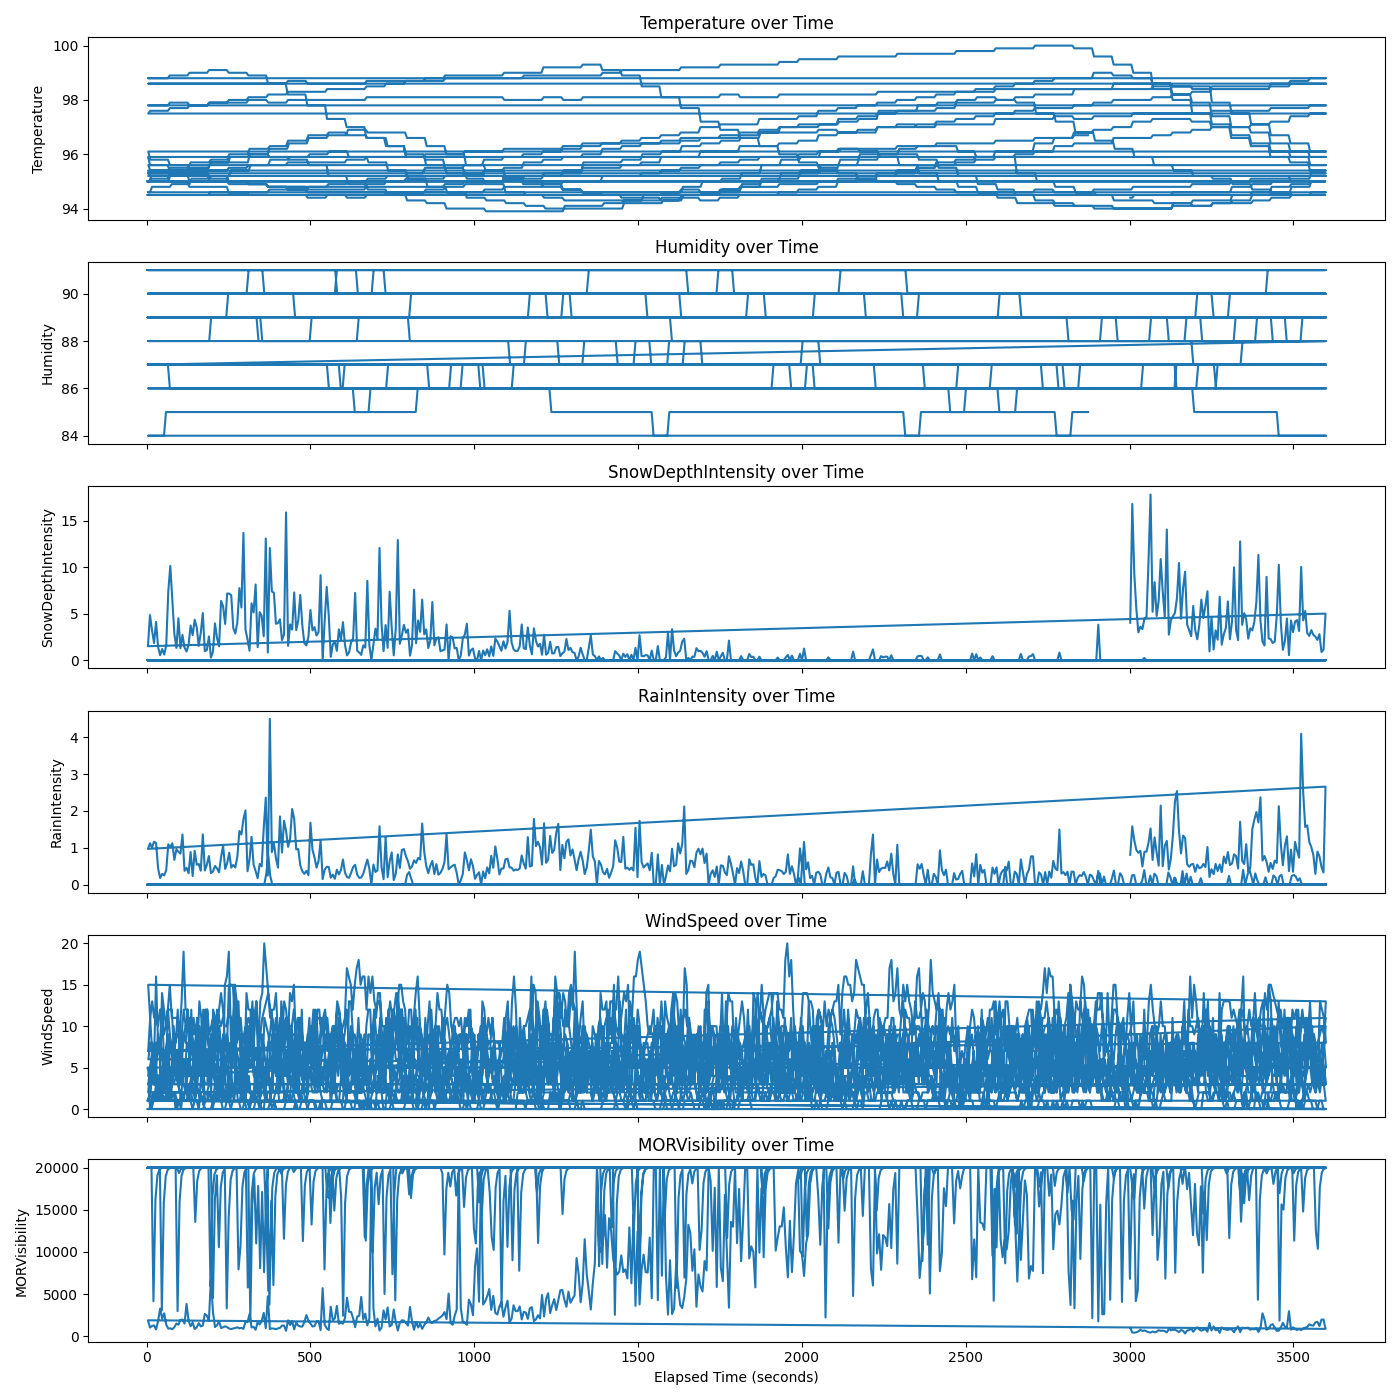
\includegraphics[width=\columnwidth]{weather_metrics_plot.png}
\caption{Repository-generated weather time series for the December 17--18 snow-session file. The source script plots temperature, humidity, snow-depth intensity, rain intensity, wind speed, and MOR visibility. Units are undocumented.}
\label{fig:weather}
\end{figure}

\section{Discussion}
The direction and magnitude of the correlations suggest that some measured weather variables co-vary with RSSI, SNR, and throughput in this dataset. However, the predictive experiments explain at most about 21\% of holdout variance, and flexible random-forest/KNN models generally do not improve performance. This pattern is consistent with weak signal, confounding by collection session or time, limited covariates, or train/test dependence; the repository cannot distinguish among these explanations.

The positive association of rain accumulators with link metrics should not be interpreted as rain improving propagation. Accumulator variables may encode time or collection-session identity, and pressure and rain measures may co-vary with unrecorded changes in geometry or hardware. Furthermore, random row splitting allows temporally adjacent, similarly averaged observations to occur in both partitions. The reported scores therefore characterize the stored pipeline, not expected performance on a new storm, site, or radio link.

\section{Limitations}
The principal limitations are: undocumented hardware and measurement units; an unknown data-collection protocol; only one identified location name (Wilson Hall) without geometry; 2,432 duplicate rows in the consolidated weather file; possible overlapping merge windows; no temporal or session-aware validation; no uncertainty intervals or multiple-testing correction; unit-mixing in averaged-feature correlations; redundant rain variables; and failed scalar interpretation of vector-valued particle fields. The scripts also use different feature sets and test fractions across targets, limiting direct model comparison. Generated images do not embed metric values or provenance, and saved console outputs are absent.

\section{Future Work}
Future work should document instruments and units, preserve explicit collection-session identifiers, decide whether repeated weather rows are valid, parse vector-valued particle distributions into justified summaries, and audit timestamp/time-zone alignment. Models should be evaluated with blocked or leave-one-session-out validation and confidence intervals. A physically motivated feature set should replace arithmetic averages across unlike units, and collinearity between cumulative rain fields should be addressed. Additional measurements across locations, distances, radio settings, and weather regimes are required before generalization.

\section{Conclusion}
This reconstruction finds reproducible but modest associations between several scalar weather measurements and LoRa RSSI, SNR, and throughput. The strongest individual correlation is $r=0.450$ between the rain accumulator fields and SNR, while latency correlations are negligible. Holdout regression performance is limited: the best tested configurations reach $R^2=0.190$ for RSSI, $0.208$ for SNR, $0.118$ for throughput, and less than zero for latency. Given missing experimental metadata, duplicated weather rows, temporal-validation concerns, and malformed vector-feature handling, the evidence supports only an exploratory conclusion: weather measurements and link metrics co-vary in the collected records, but neither causal effects nor robust out-of-session prediction have been established.


\section*{Acknowledgment}
\textbf{TODO:} Add funding, institutional, equipment, and contributor acknowledgments.

\section*{References}
\textbf{TODO:} Add verified references after completing the literature review. The accompanying \texttt{references.bib} is intentionally empty to avoid fabricated citations.

\appendices
\section{Repository Audit Notes}
The source audit covered all 12 Python files, 18 CSV files, two Excel workbooks, 20 PNG figures, the backup source listing, and project metadata. No notebooks, PDFs, LaTeX manuscripts, formal reports, presentations, or saved console logs were present. The empty file \texttt{merged\_lora\_weather.csv} was not used.

\end{document}
